\documentclass[refman]{scrartcl}

\usepackage[english]{babel}
\usepackage[utf8]{inputenc}

\usepackage{fancyhdr}
\usepackage{graphicx}
\usepackage[dvipsnames]{xcolor} 
\usepackage{epigraph}


\usepackage{amsmath}

\usepackage{listings}

\pagestyle{fancy}

\lstdefinestyle{mystyle}{
    backgroundcolor=\color{white},   
    commentstyle=\color{codegreen},
    keywordstyle=\color{Fuchsia},
    numberstyle=\tiny\color{gray},
    stringstyle=\color{codepurple},
    basicstyle=\footnotesize,
    breakatwhitespace=false,         
    breaklines=true,                 
    captionpos=b,                    
    keepspaces=true,                 
    numbers=left,                    
    numbersep=5pt,                  
    showspaces=false,                
    showstringspaces=false,
    showtabs=false,                  
    tabsize=2
}
 
\lstset{style=mystyle}


\newcommand{\mymod}{\text{\ \ mod\ \ }}

\begin{document}

% ----------------------------------------------------------------------------------------------------------
% PREAMBLE
% ----------------------------------------------------------------------------------------------------------

\begin{titlepage}
	\centering
	
\includegraphics[width=0.15\textwidth]{graphics/huberlin_logo}\par\vspace{1cm}
	{\scshape\LARGE Humboldt University of Berlin \par}
	\vspace{1cm}
	{\scshape\Large Einf{\"u}hrung in das wissenschaftliche Rechnen \par}
	\vspace{1.5cm}
	{\huge\bfseries Documentation of Fraction Application Programming Interface and Command Line Interface Calculator\par}
	\vspace{2cm}
	{\Large\itshape Christian Parpart \& Kei Thoma \par}
	\vfill

	\vfill

% Bottom of the page
	{\large \today\par}
\end{titlepage}

\tableofcontents
\newpage

% ----------------------------------------------------------------------------------------------------------
% CONTENTS
% ----------------------------------------------------------------------------------------------------------

\section{Introduction: Complexity One Horizon}
\vspace{4cm}\epigraph{“Life is really simple, but we insist on making it complicated."}{\textit{Confucius}}

\noindent Our goal was to write a proper fraction calculator. For that, however, we needed to implement the Euclidean algorithm which computes the greatest common divisor. This algorithm is admittingly fast, but certainly not \(\mathcal{O}(1)\) fast \cite{knuth}. So we coded one. Greatest common divisor at complexity one.

This was done by precomputing all greatest common divisor from 1 to n and saving the results to a local file. While the Euclidean algorithm often needs multiple iterations to find the solution, looking up a value is always a single step.
% ----------------------------------------------------------------------------------------------------------
% EUCLIDEAN ALGORITHM LIBRARY
% ----------------------------------------------------------------------------------------------------------

\section{tools3 Library}

The goal of this module is to implement the Euclidean algorithm, which finds the greatest common divisor, with complexity O(1). This is realized by precomputing (iteratively) all greatest common divisor from 1 to n.

We have left another (recursive) version of the algorithm in the module in case of an emergency.

Lastly, this module includes a function to calculate the least common multiple with the help of the aforementioned Euclidean algorithm.

\subsection{class GreatestCommonDivisor}

This class implements the Euclidean algorithm with ensuring that smaller greatest common divisors have complexity O(1), by precomputing all greatest common divisors between 1 and n (with n being chosen at the constructor). The precomputed greatest common divisors are stored in a local file for faster instantiation later.

\subsubsection{def \_\_init\_\_(\_filename, \_dim)}

\paragraph*{Arguments}

\begin{enumerate}
	\item \_filename (string): the file name
	\item \_dim (int): the largest number to precomputed
\end{enumerate}

\paragraph*{Description}

Constructing the greatest common divisor object by either optionally precomputing all greatest common divisor between 1 and \_dim, and writes them to disk (\_filename) for future acess.

\subsubsection{def compute(\_a, \_b)}

\paragraph*{Arguments}

\begin{enumerate}
	\item \_a (int): the fist integer
	\item \_b (int): the second integer
\end{enumerate}

\paragraph*{Returns}

\begin{itemize}
	\item (int): the result of the Euclidean algorithm of \_a and \_b
\end{itemize}

\paragraph*{Description}

She returns the result of the Euclidean algorithm by actually iteratively computing.

\subsubsection{def write\_cache(self)}

\paragraph*{Returns}

\begin{itemize}
	\item None
\end{itemize}

\paragraph*{Description}

Member method to populate a cache for O(1) access.
Internally, this function calls the class method write\_cache\_to
with the respective parameters.

\subsubsection{def write\_cache\_to(\_filename, \_dim)}

\paragraph*{Arguments}

\begin{itemize}
	\item \_filename: Local file systems file name to write the cache to.
	\item \_dim: Highest number the cache will pre-compute the GCD for.
\end{itemize}

\paragraph*{Returns}

\begin{itemize}
	\item Nothing
\end{itemize}

\paragraph*{Description}

This class method can be used to create a fresh cache of precomputed GCD values from 1 to \_dim for both input parameters of gcd.

\subsubsection{def gcd(self, \_a, \_b)}

\paragraph*{Arguments}

\begin{enumerate}
	\item \_a (int): the fist integer
	\item \_b (int): the second integer
\end{enumerate}

\paragraph*{Returns}

\begin{itemize}
	\item (int): the greatest common divisor of \_a and \_b
\end{itemize}

\paragraph*{Description}

Computes GCD of a and b either in O(1) complexity if in range of precomputation, or iteratively.

\subsection{Free Functions}

\subsubsection{def recursive\_euclidean\_algorithm(a, b)}

\paragraph*{Arguments}

\begin{enumerate}
  \item \texttt{first\_number} (int): the first integer, \textit{a}; negative values are accepted
  \item \texttt{second\_number} (int): the second integer, \textit{b}; negative values are accepted
\end{enumerate}

\paragraph*{Returns}

\begin{itemize}
  \item (int): the greatest common divisor found via the recursive euclidean algorithm
\end{itemize}

\paragraph*{Description}

\begin{figure}
	\centering
		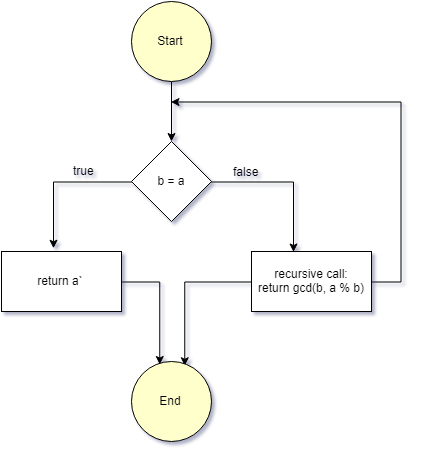
\includegraphics[width=0.5\textwidth]{graphics/recursive_euclidean_algorithm}
	\caption{The recursive Euclidean algorithm}\label{fig:recursive}
  \end{figure}

Given two integers, she finds the greatest common divisor via the recursively implemented euclidean algorithm (for the validity of the algorithm see \cite{bosch}).

The algorithm itself starts with two integers \(a\) and \(b\). If \(b = 0\) then \(a\) is returned and the recursive loop stops. In any other case, this function is called again, but the arguments are modified in the following manner
%
\begin{align*}
	b \mapsto \text{first argument} \hspace{3cm} a \mymod b \mapsto \text{second argument} \text{,}
\end{align*}
%
or if one prefers to read the statement in code (see also figure \ref{fig:recursive})
%
\begin{lstlisting}[language=Python]
def euclidean_algorithm(a, b):
return a if b_5 == 0 else euclidean_algorithm(b, a % b)
\end{lstlisting}

\paragraph*{Worked Example of the Algorithm}

Let \(a = 195\) and \(b = 1287\). Following the algorithm above, we have
%
\begin{center}
	\begin{tabular}{ l l l l }
	 Step 0 & \(a_0 = 195\) & \(b_0 = 1287\) & \\ 
	 Step 1 & \(a_1 = 1287\) & \(b_1 = 195 \mymod 1287\) & \(= 195\) \\  
	 Step 2 & \(a_2 = 195\) & \(b_2 = 1287 \mymod 195\) & \(= 117\) \\
	 Step 3 & \(a_3 = 117 \) & \(b_3 = 195 \mymod 117\) & \(= 78\) \\
	 Step 4 & \(a_4 = 78\) & \(b_4 = 117 \mymod 78\) & \(= 39\)\\
	 Step 4 & \(a_5 = 39\) & \(b_5 = 78 \mymod 39\) & \(= 0\)
	\end{tabular}
\end{center}
%
Since \(b = 0\), the algorithm is stopped and \(a_5 = 39\) is returned.

\subsubsection{def least\_common\_multiple(a, b)}

\paragraph*{Arguments}

\begin{enumerate}
  \item \texttt{first\_number} (int): the first integer, \textit{a}; negative values are accepted
  \item \texttt{second\_number} (int): the second integer, \textit{b}; negative values are accepted
\end{enumerate}

\paragraph*{Returns}

\begin{itemize}
  \item (int): the least common multiple calculated with the help of the euclidean algorithm and the formula
\end{itemize}

\paragraph*{Description}

She calculates the least common multiple using the result of the euclidean algorithm and the following formula (for the validity of the formula see \cite{bosch})
%
\[\text{lcm}(a, b) = \frac{|a \cdot b|}{\text{gcd}(a, b)} \text{.}\]

\subsubsection{def main()}

\paragraph*{Returns}

\begin{itemize}
	\item None
\end{itemize}

\paragraph*{Description}

The main function for testing purposes. She prints out some greatest common divisors and least common multiples into the console.

% ----------------------------------------------------------------------------------------------------------
% FRACTION API
% ----------------------------------------------------------------------------------------------------------

\section{Fraction API}

The Fraction class in \texttt{fraction.py} implements a fraction, i.e. concepts such as \(\frac{1}{2}\) or \(-\frac{2}{3}\), mathematically correctly. For this endeavor, Fraction saves three pseudo-private attributes representing the unsigned numerator, the unsigned denominator and finally the sign of the fraction.

After an instance of Fraction is initialized, it is automatically reduced properly to the most minimal form, e.g. \(\frac{8}{12}\) naturally becomes \(\frac{2}{3}\), with the help of the euclidean algorithm.

Finally, to allow some easy way to handle this class, few build-in operators such as the absolute function and binary addition were overloaded.

\subsection{Attributes}

\begin{itemize}
	\item numerator\_ (int): the unsigned numerator of the fraction instance
	\item denominator\_ (int): the unsigned denominator of the fraction instance
	\item sign\_ (boolean): the sign of the fraction instance; this should be False if the fraction is positive or zero and should be True if the fraction is negative
\end{itemize}

\subsection{def \_\_init\_\_(numerator, denominator)}

\subsubsection*{Arguments}

\begin{enumerate}
  \item \texttt{numerator} (int): the numerator; negative values are allowed, but is then saved as a positive integer at \texttt{numerator\_}
  \item \texttt{denominator} (int): the denominator; negative values are allowed, but is then saved as a positive integer at \texttt{denominator\_}; if no argument is passed, it defaults to 1
\end{enumerate}

Note that even though \texttt{numerator\_} and \texttt{denominator\_} are always positive, the sign of the Fraction is determined at the point of initalization and is saved under the boolean attribute \texttt{sign\_}.

\subsubsection*{Raises}

\begin{itemize}
  \item \texttt{ZeroDivisionError}: if \(0\) is passed as the parameter for the denominator
\end{itemize}

\subsubsection*{Description}

The constructor initializes the fraction object with the given numerator and denominator. As mentioned before, the sign of the fraction is saved separately as a boolean (True for negative, False for positive fractions and zero). 

\subsection{def reduce\_fraction\_(self)}

\subsubsection*{Returns}

\begin{itemize}
	\item None
\end{itemize}

\subsubsection*{Description}

She is a private function and as such should only be used inside this class. When called, she finds the greatest common denominator with the Euclidean algorithm (implemented in \texttt{euclidean\_algorithm.py}) and divides the attributes numerator\_ and denominator\_ with this result reducing the fraction.

\subsection{def sgn\_(self)}

\subsubsection*{Returns}

\begin{itemize}
	\item (int): -1 if the sign\_ is True and 1 if it is False
\end{itemize}

\subsubsection*{Description}

A little auxilary function which returns the numerical value of the sign (-1 or 1). She is used in other methods to apply the sign in calculations

\subsection{Get Attribute Functions}

\subsubsection*{Returns}

\begin{itemize}
	\item (int) or (boolean): the respective attribute of the fraction object
\end{itemize}

\subsubsection*{Description}

Fortunataly or unfortunataly depending on one's perspective about dynamic languages, Python does not allow private attributes or methods. However, we don't want that the three attributes, \texttt{numerator\_}, \texttt{denominator\_}, and \texttt{sign\_}, are modifiable from the outside of the Fraction class. Therefore, this class provides three methods, \texttt{get\_numerator()}, \texttt{get\_denominator()}, and \texttt{get\_sign()}, which simply returns the respective attribute.

\subsection{def \_\_pos\_\_(self)}

\subsubsection*{Returns}

\begin{itemize}
  \item (self): returns the unchanged self
\end{itemize}

\subsubsection*{Description}

Overloading the unary plus operator is not very exciting. The fraction object is unchanged and returned immediately.

\subsection{def \_\_neg\_\_(self)}

\subsubsection*{Returns}

\begin{itemize}
	\item (self): returns self, but negates the sign, i.e. True becomes False and False becomes True; if the numerator was 0, the sign is unchanged
  \end{itemize}

\subsubsection*{Description}

A little more exciting than the unary plus. This function changes the \texttt{sign\_} to True if the fraction was positive and to False if the fraction was negative. If the numerator was 0, she returns self without changing the sign.

\subsection{def \_\_abs\_\_(self)}

\subsubsection*{Returns}

\begin{itemize}
	\item (self): returns self, but the sign is changed to False
\end{itemize}

\subsubsection*{Description}

To determine the absolute value of the fraction, she either returns the object unchanged if the fraction was already negative or uses the \texttt{\_\_neg\_\_()} to return the positive fraction.

\subsection{def \_\_add\_\_(self, other)}

\subsubsection*{Arguments}

\begin{enumerate}
	\item self (Fraction): the fraction on the right side; first summand
	\item other (Fraction): the fraction on the left side; second summand
\end{enumerate}

\subsubsection*{Returns}

\begin{itemize}
	\item (Fraction): the sum of self and other as a new instance of the Fraction class
\end{itemize}

\subsubsection*{Description}

This magic method overloads the binary infix plus and returns the sum of two fractions as a new instance. The new fraction is calculated in the following manner
%
\begin{equation}
	\frac{a}{b} + \frac{c}{d} = \frac{ad + bc}{bd} \text{.}
\end{equation}
%
She does not need to find the greatest common denominator here, because the new Fraction will be reduced properly at the constructor.

\subsection{def \_\_sub\_\_(self, other)}

\subsubsection*{Arguments}

\begin{enumerate}
	\item self (Fraction): the fraction on the right side; the subtrahend
	\item other (Fraction): the fraction on the left side; the minuend
\end{enumerate}

\subsubsection*{Returns}

\begin{itemize}
	\item (Fraction): the difference of self and other as a new instance of the Fraction class
\end{itemize}

\subsubsection*{Description}

The antithesis of the binary infix plus operation. As such, she uses the binary plus in conjuction with the unary negative to return the difference of the two given fraction as a new fraction object.

\subsection{def \_\_mul\_\_(self, other)}

\subsubsection*{Arguments}

\begin{enumerate}
	\item self (Fraction): the fraction on the right side; the first factor
	\item other (Fraction): the fraction on the left side; the second factor
\end{enumerate}

\subsubsection*{Returns}

\begin{itemize}
	\item (Fraction): the product of self and other as new instance of the Fraction class
\end{itemize}

\subsubsection*{Description}

She overloads the binary infix multiplication for the Fraction objects. For the calculation, this formula is used

\begin{equation}
	\frac{a}{b} \cdot \frac{c}{d} = \frac{ac}{bd} \text{.}
\end{equation}

Again, we do not need to reduce here, because the magic is taken care at initalization.

\subsection{def \_\_str\_\_(self)}

\subsubsection*{Returns}

\begin{itemize}
	\item (string): the format of the string is \texttt{a/b}
\end{itemize}

This function returns the attributes of a Fraction instance as a readable string. The \texttt{print()} function uses her to print the Fraction object neatly to the console.

\subsection{def summe(self, \_rhs)}

\subsubsection*{Arguments}
\begin{itemize}
	\item self (Fraction): the left hand side of the fractional addition operation.
	\item \_rhs (Fraction): the right hand side of the fractional addition operation.
\end{itemize}

\subsubsection*{Returns}
\begin{itemize}
	\item Fraction: The sum of two fractional numbers in reduced representation.
\end{itemize}

\subsubsection*{Description}
This method implements the fractional addition operation
with the object itself being the left hand side
and \_rhs being the right hand side of this operation.

\subsection{def main()}

\subsubsection*{Returns}

\begin{itemize}
	\item None
\end{itemize}

\subsubsection*{Description}

The main function for testing purposes. She prints every magic methods which was defined in the class.

\section{Fraction Calculator CLI}

\subsection{def interpret(user\_input)}

\subsubsection*{Arguments}

\begin{enumerate}
	\item user\_input (string): the string entered to the console by the user
\end{enumerate}

\subsubsection*{Returns}

\begin{itemize}
	\item (Fraction): the Fraction object constructed by the user's input
\end{itemize}

\subsubsection*{Description}

This function constructs a fraction object according to the string passed.

\subsection{def main()}

\subsubsection*{Returns}

\begin{itemize}
	\item None
\end{itemize}

\subsubsection*{Description}

The main function of the fraction calculator. When called, the user is asked to input two fraction and their sum is printed on the console. The user can then exit the module by typing any word starting with an n to exit.

\section{Fraction Calculator Manual}

The calculator currently adds two fraction together. Simply start the module, type fractions each in a new line and seperate the numerator and denominator with a slash /. The solution should then be printed on the console.

Figure \ref{fig:example} shows the output of the calculator with the user input being \(\frac{1}{2}\) and \(\frac{-1}{3}\). After the user has input two fraction, the sum, here \(\frac{1}{6}\), is printed.

\begin{figure}[h]
	\centering
		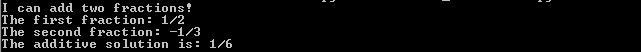
\includegraphics[width=0.9\textwidth]{graphics/calculator_example}
	\caption{example of the output of the fraction calculator}\label{fig:example}
\end{figure}

\section{Future Improvements}

One of our immediate goals in the comming future would be to equip the currently limited fraction calculator with more arithmetic options such as subtraction or power. The latter would require an expansion to the fraction class.

\begin{thebibliography}{9}
	\bibitem{bosch} 
	Bosch, Siegfried. 
	\textit{Algebra}. 
	Springer-Verlag Berlin Heidelberg, 7th Edition, 2009.
	
	\bibitem{knuth} 
	Knuth, Donald. 
	\textit{The Art of Computer Programming Volume 2}. 
	Prentice Hall, 3rd Edition, 1997.
	
\end{thebibliography}

\end{document}
